\section{Wechselstromschalter, Wechselstromsteller und Gleichstromsteller}

Leistungselektronische Stellglieder lassen sich in Wechselstromschalter,
Wechselstromsteller und Gleichstromsteller einteilen.
Sie unterscheiden sich durch die Art der Spannung, die Stellgrösse
und die verwendete Schaltfrequenz.

% =========================================================
\subsection{Wechselstromschalter}

% --- bestehende Grafik ---
Wechselstromschalter mit bidirektionalem Ventil
\begin{center}
    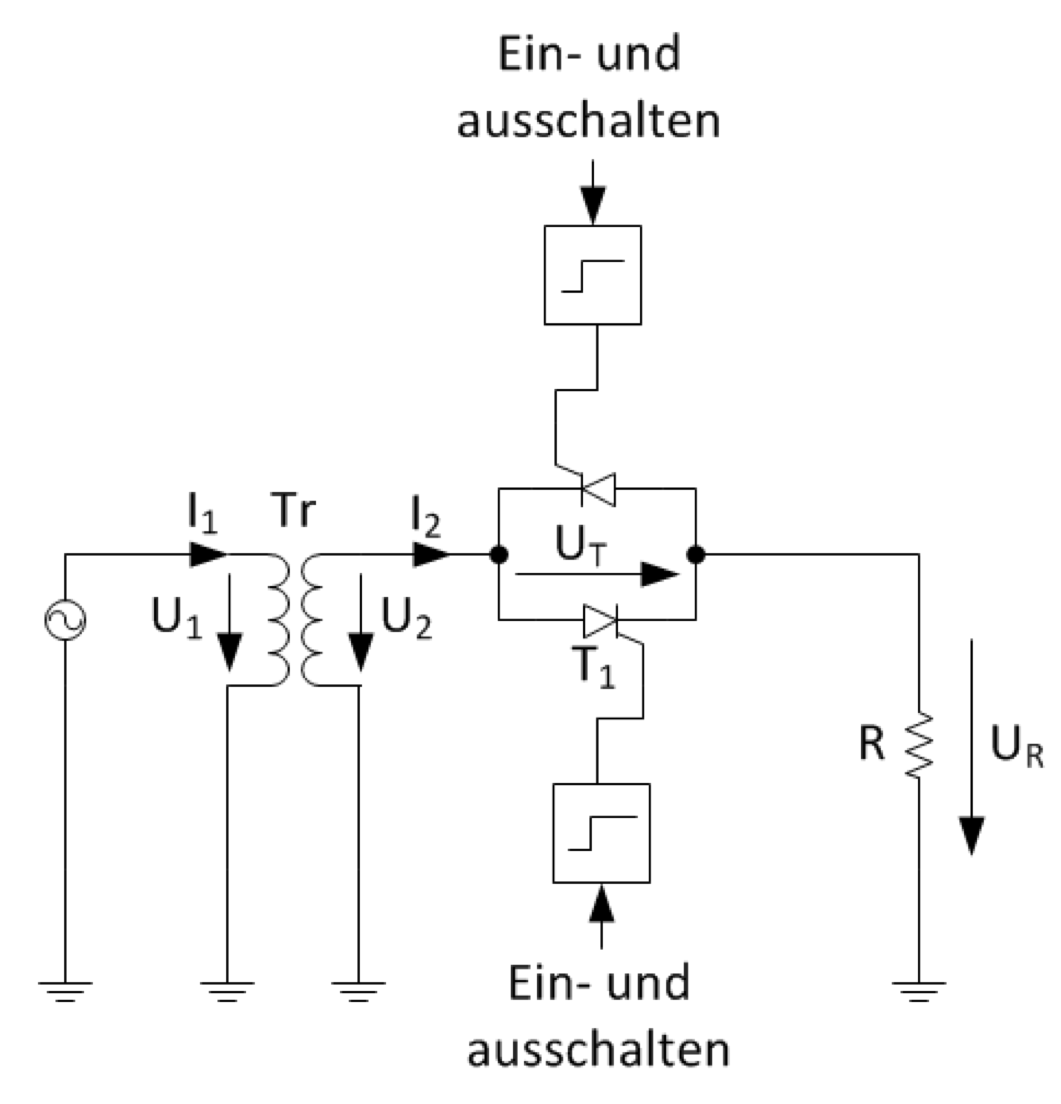
\includegraphics[width=0.85\linewidth]{images/Wechselstromschalter.png}
\end{center}

Ein Wechselstromschalter dient ausschließlich zum Ein- und Ausschalten einer Wechselspannung.
Er verändert weder die Spannungsform noch den Effektivwert, sondern schaltet die Last lediglich zu oder ab.
Die Steuerung erfolgt binär, ohne Stellfunktion.
Typische Anwendungen sind Netzschütze, Relais und einfache Netzschalter.
Wechselstromschalter sind keine Steller.

Schaltgleichung:
\[
u_L(t)=
\begin{cases}
u_s(t), & \text{Schalter geschlossen},\\
0, & \text{Schalter offen}.
\end{cases}
\]

mit:
\begin{itemize}
\item $u_s(t)$: Eingangsspannung,
\item $u_L(t)$: Lastspannung.
\end{itemize}

% =========================================================
\subsection{Wechselstromsteller (Phasenanschnittsteller)}

% --- bestehende Grafik ---
Phasenanschnittsteuerung beim Wechselstromsteller
\begin{center}
    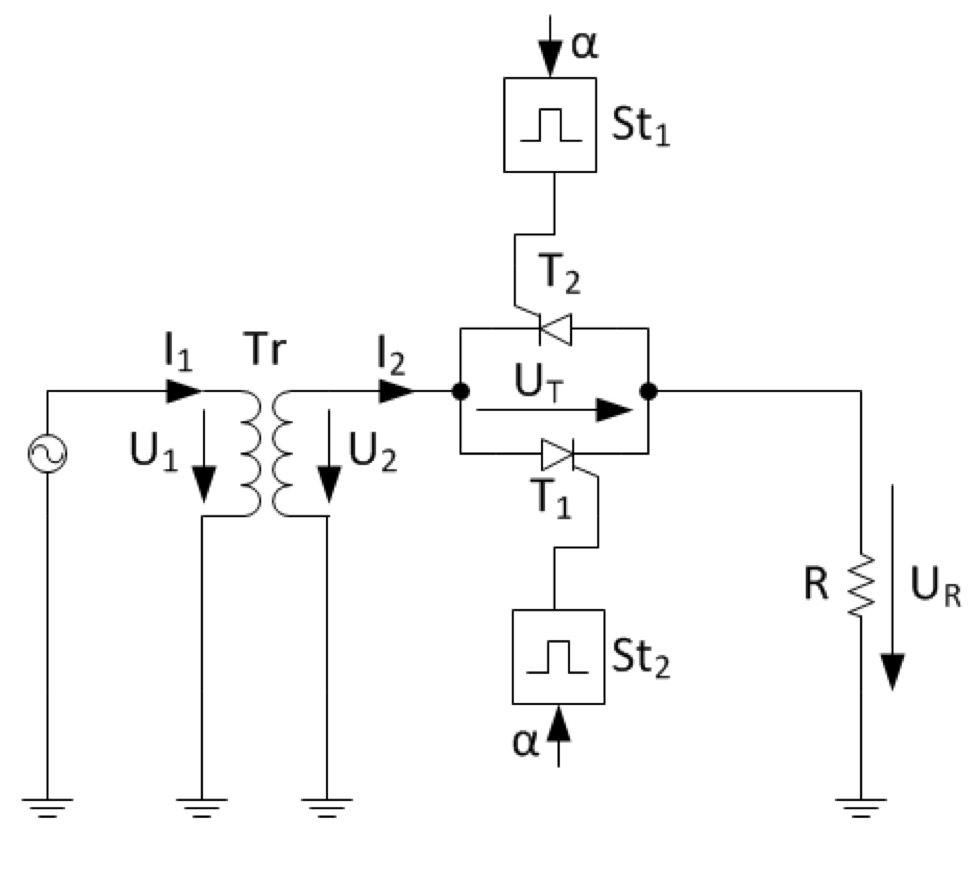
\includegraphics[width=0.85\linewidth]{images/Wechselstromsteller.png}
\end{center}

Ein Wechselstromsteller erzeugt aus einer konstanten Wechselspannung eine stellbare Wechselspannung
durch Phasenanschnittsteuerung.
Der Leitbeginn wird über den Zündwinkel $\alpha$ festgelegt.
Die Ausgangsspannung ist nicht sinusförmig und enthält starke Oberschwingungen.
Die Regelung erfolgt mit Netzfrequenz.
Typische Anwendungen sind Lichtdimmer und Heizleistungssteller.

Eingangsspannung:
\[
u_s(t)=\hat U \sin(\omega t)
\]

mit:
\begin{itemize}
\item $\hat U$: Scheitelwert,
\item $U_s=\hat U/\sqrt{2}$: Effektivwert der Eingangsspannung,
\item $\omega=2\pi f$: Kreisfrequenz,
\item $f$: Netzfrequenz.
\end{itemize}

Momentane Ausgangsspannung:
\[
u(t)=
\begin{cases}
\hat U\sin(\omega t), & \omega t \ge \alpha,\\
0, & \omega t < \alpha.
\end{cases}
\]

\paragraph{R-Last}

Effektivwert:
\[
\boxed{
U_{\mathrm{RMS}}(\alpha)
=U_s\sqrt{\frac{1}{\pi}\int_{\alpha}^{\pi}\sin^2\theta\,d\theta}
}
\]

Geschlossene Form:
\[
\boxed{
U_{\mathrm{RMS}}(\alpha)
=U_s\sqrt{\frac{1}{2\pi}\left(\pi-\alpha+\frac{1}{2}\sin 2\alpha\right)}
}
\]

Strom:
\[
\boxed{I_{\mathrm{RMS}}(\alpha)=\frac{U_{\mathrm{RMS}}(\alpha)}{R}}
\]

Wirkleistung:
\[
\boxed{P(\alpha)=\frac{U_{\mathrm{RMS}}^2(\alpha)}{R}}
\]

Mittelwert der Ausgangsspannung:
\[
\boxed{
\overline{u}(\alpha)=\frac{1}{2\pi}\int_{\alpha}^{\pi}\hat U\sin\theta\,d\theta
=\frac{\hat U}{2\pi}(1+\cos\alpha)
}
\]

\paragraph{R--L-Last}

Differentialgleichung im Leitintervall:
\[
L\frac{di}{dt}+Ri=\hat U\sin(\omega t)
\]

Allgemeine Lösung:
\[
\boxed{
i(t)=C e^{-t/\tau}+\frac{\hat U}{Z}\sin(\omega t-\varphi)
}
\]

mit:
\[
\tau=\frac{L}{R},\qquad
Z=\sqrt{R^2+(\omega L)^2},\qquad
\tan\varphi=\frac{\omega L}{R}
\]

Löschwinkel:
\[
\boxed{i(\beta)=0}
\]

Leitbedingung:
\[
\boxed{\alpha<\beta}
\]

Eigenschaften:
\begin{itemize}
\item Stellgrösse: Zündwinkel $\alpha$,
\item Nichtsinusförmige Spannung und Strom,
\item Starke Netzstromharmonische,
\item Schlechter Leistungsfaktor bei kleinem $\alpha$.
\end{itemize}

% =========================================================
\subsection{Gleichstromsteller (Chopper)}

Ein Gleichstromsteller wandelt eine konstante Gleichspannung $U_{DC}$
in eine stufenlos einstellbare Gleichspannung $u_d$
durch schnelles periodisches Ein- und Ausschalten eines Halbleiterschalters.
Die Stellgrösse ist der Tastgrad $d$.
Der Schalter arbeitet mit hoher Schaltfrequenz $f_s$.
Im kontinuierlichen Betrieb entspricht der Gleichstromsteller einem Buck-Wandler.
Er ist das Standard-Stellglied für Gleichstromantriebe.

% -------------------------------------------------
\subsubsection{Grundgrössen und Definitionen}

Tastgrad:
\[
\boxed{d=\frac{t_{\mathrm{on}}}{T_s}}, 
\qquad
T_s=\text{Schaltperiode}, 
\qquad
f_s=\frac{1}{T_s}
\]

Mittelwert der Ausgangsspannung (CCM):
\[
\boxed{u_d=d\,U_{DC}}
\]

Effektivwert der Ausgangsspannung (ideales PWM-Rechteck):
\[
\boxed{U_{d,\mathrm{RMS}}=U_{DC}\sqrt{d}}
\]

mit:
\begin{itemize}
\item $U_{DC}$: Eingangsgleichspannung,
\item $u_d$: mittlere Ausgangsspannung,
\item $U_{d,\mathrm{RMS}}$: Effektivwert der Ausgangsspannung,
\item $t_{\mathrm{on}}$: Einschaltzeit,
\item $T_s$: Schaltperiode,
\item $f_s$: Schaltfrequenz.
\end{itemize}

Ausgangsleistung (ideal):
\[
\boxed{P_{\mathrm{out}}=u_d\,I_d}
\]

% -------------------------------------------------
\subsubsection{R--L-Last im Zeitbereich}

Lastgleichung:
\[
L\frac{di}{dt}+Ri=u_d(t)
\]

Zeitkonstante:
\[
\boxed{\tau=\frac{L}{R}}
\]

\paragraph{EIN-Phase ($0<t<t_{\mathrm{on}}$)}

\[
L\frac{di}{dt}+Ri=U_{DC}
\]

\[
\boxed{
i(t)=\frac{U_{DC}}{R}
+\left(i_{\min}-\frac{U_{DC}}{R}\right)e^{-t/\tau}
}
\]

\paragraph{AUS-Phase ($t_{\mathrm{on}}<t<T_s$)}

\[
L\frac{di}{dt}+Ri=0
\]

\[
\boxed{
i(t)=i_{\max}e^{-t/\tau}
}
\]

Periodenbedingung:
\[
\boxed{i_{\min}=i_{\max}e^{-T_a/\tau}}, 
\qquad T_a=T_s-t_{\mathrm{on}}
\]

% -------------------------------------------------
\subsubsection{Induktorspannung und Mittelwertbedingung}

Induktorspannung:
\[
u_L(t)=L\frac{di}{dt}
\]

Stationärer Betrieb:
\[
\boxed{\overline{u_L}=0}
\]

Daraus folgt direkt:
\[
\boxed{u_d=d\,U_{DC}}
\]

Dies ist die fundamentale Mittelwertbedingung des Gleichstromstellers.

% -------------------------------------------------
\subsubsection{Stromrippel und Betriebsarten}

Stromrippel:
\[
\boxed{\Delta i=i_{\max}-i_{\min}}
\]

Während EIN:
\[
\boxed{
\Delta i_{\mathrm{on}}\approx\frac{(U_{DC}-u_d)}{L}\,dT_s
}
\]

Während AUS:
\[
\boxed{
\Delta i_{\mathrm{off}}\approx\frac{u_d}{L}\,(1-d)T_s
}
\]

Stationär:
\[
\boxed{\Delta i=\Delta i_{\mathrm{on}}=\Delta i_{\mathrm{off}}}
\]

\paragraph{Grenzbetrieb CCM/DCM}

Grenzstrom:
\[
\boxed{I_{d,\mathrm{gr}}=\frac{\Delta i}{2}}
\]

Grenzinduktivität:
\[
\boxed{
L_{\min}=\frac{(1-d)R}{2f_s}
}
\]

\begin{itemize}
\item $L>L_{\min}$: kontinuierlicher Betrieb (CCM),
\item $L<L_{\min}$: diskontinuierlicher Betrieb (DCM),
\item DCM: $u_d=dU_{DC}$ gilt nicht mehr exakt.
\end{itemize}

% -------------------------------------------------
\subsubsection{Schalter- und Diodenbelastung}

Schalterstrom:
\[
i_S(t)=
\begin{cases}
i(t), & 0<t<t_{\mathrm{on}},\\
0, & t_{\mathrm{on}}<t<T_s
\end{cases}
\]

Diodenstrom:
\[
i_D(t)=
\begin{cases}
0, & 0<t<t_{\mathrm{on}},\\
i(t), & t_{\mathrm{on}}<t<T_s
\end{cases}
\]

Mittelwerte:
\[
\boxed{
I_{S,\mathrm{avg}}=d\,I_d,
\qquad
I_{D,\mathrm{avg}}=(1-d)\,I_d
}
\]

Effektivwerte (kleiner Rippel):
\[
\boxed{
I_{S,\mathrm{RMS}}\approx\sqrt{d}\,I_d,
\qquad
I_{D,\mathrm{RMS}}\approx\sqrt{1-d}\,I_d
}
\]

% =========================================================
\subsubsection{Einquadrantensteller (1Q)}

% --- bestehende Grafik ---
\begin{center}
    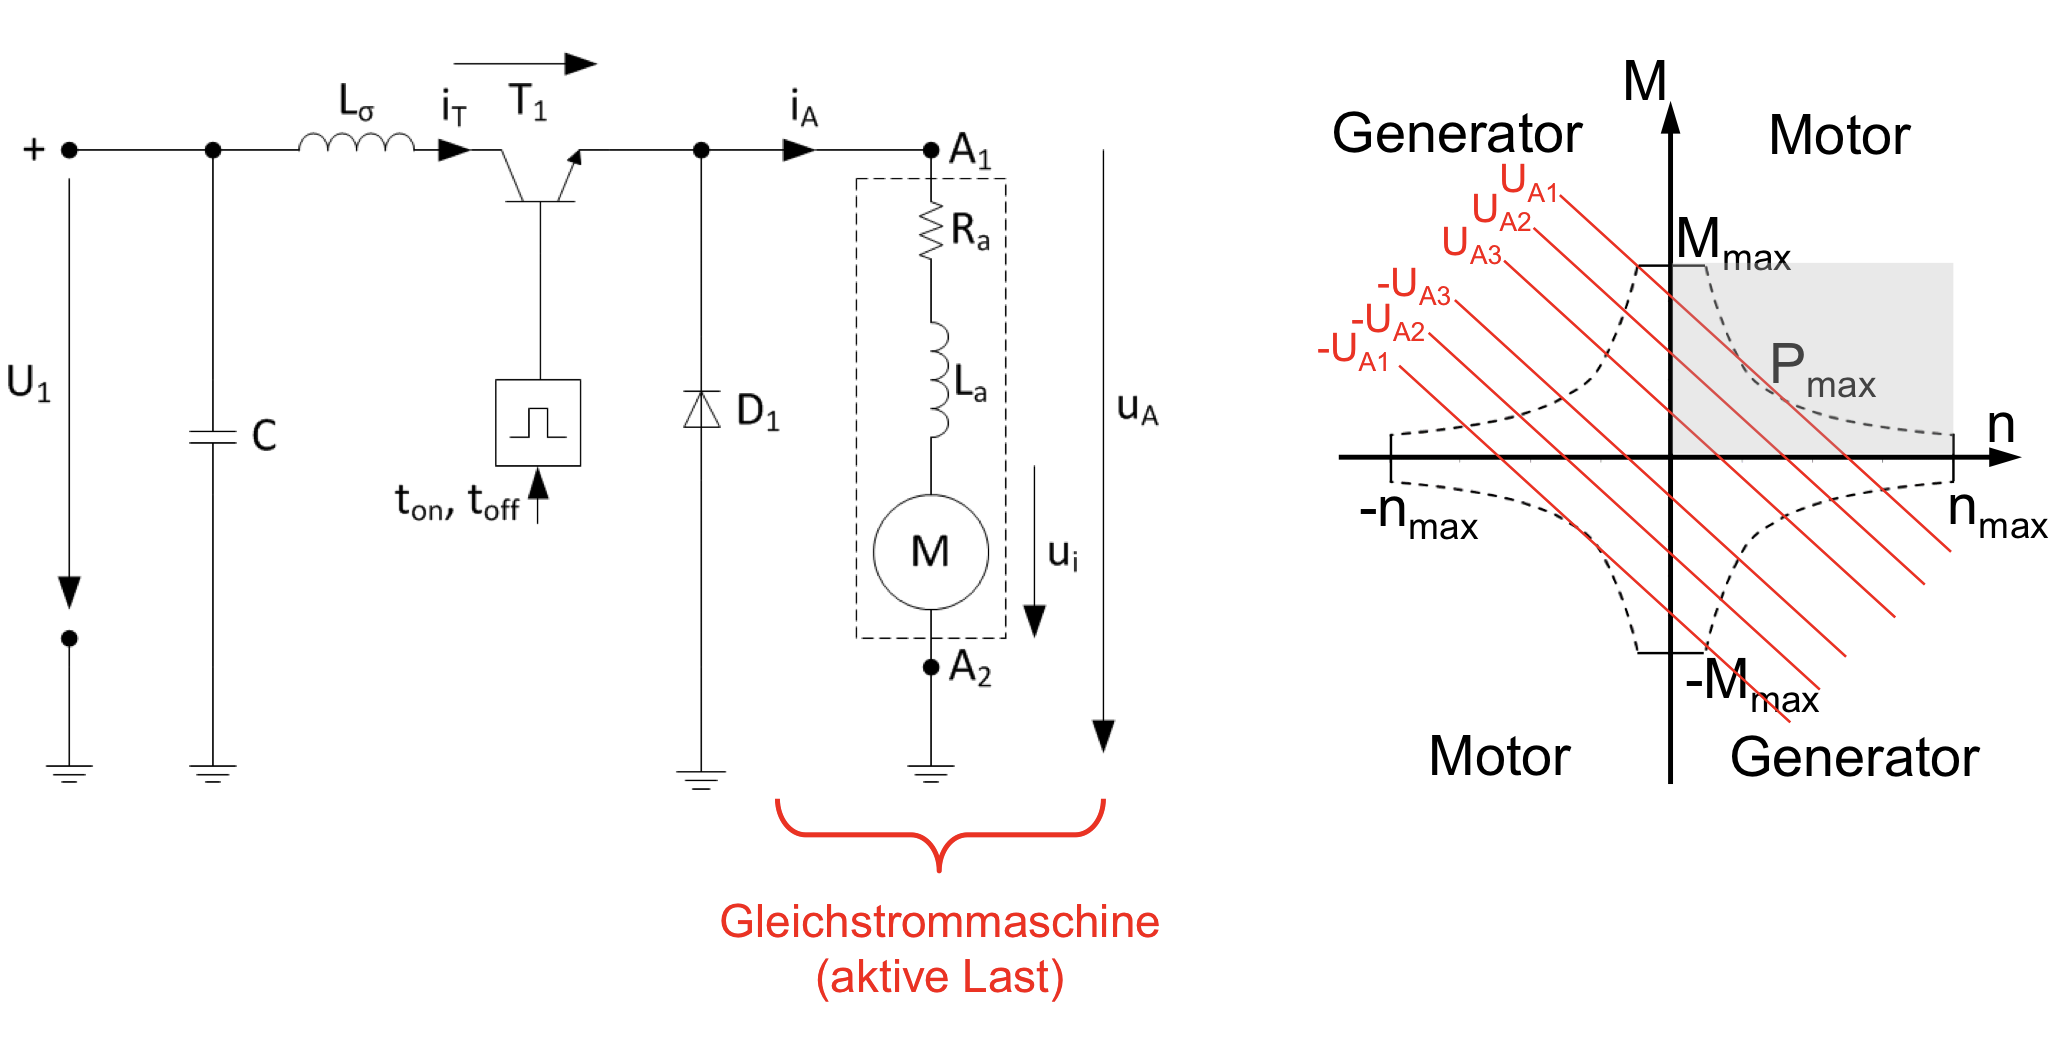
\includegraphics[width=0.85\linewidth]{images/Gleichstromsteller1Q.png}
\end{center}

Der Einquadrantensteller erlaubt nur positive Spannung und positiven Strom.
Er arbeitet ausschließlich im Motorbetrieb vorwärts.
Energie kann nur von der Quelle zur Last fliessen.
Eine Rückspeisung ist nicht möglich.
Dies ist die einfachste und am häufigsten eingesetzte Chopper-Topologie.

Betriebsbereich:
\[
\boxed{u_d\ge 0,\qquad i_d\ge 0,\qquad P=u_d i_d>0}
\]

Spannungssteuerung:
\[
\boxed{u_d=d\,U_{DC}}
\]

% =========================================================
\subsubsection{Zweiquadrantensteller (2Q)}

% --- bestehende Grafik ---
\begin{center}
    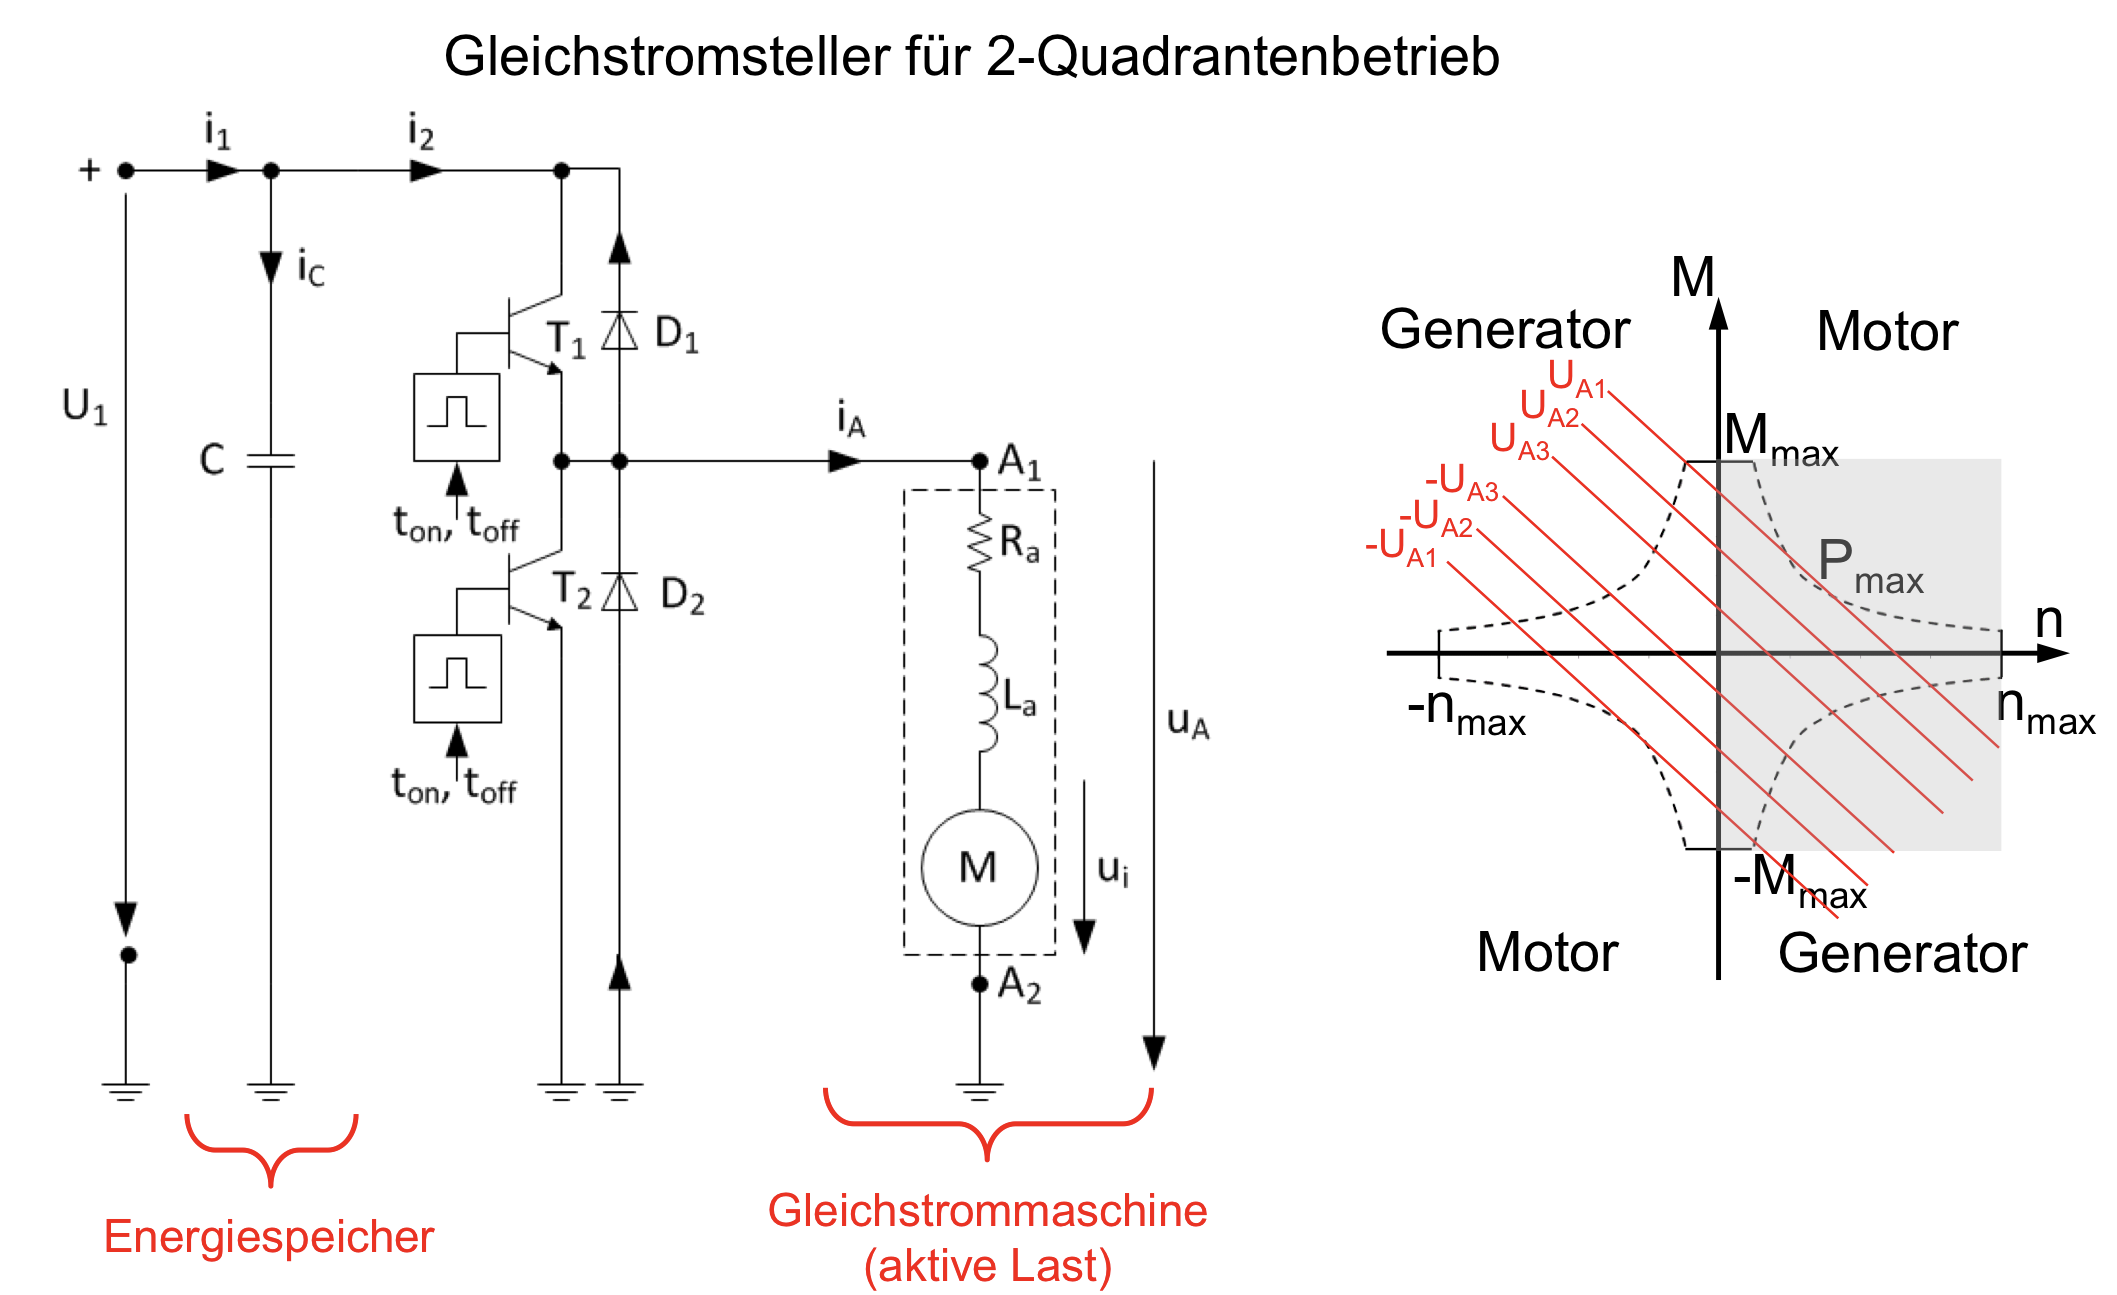
\includegraphics[width=0.85\linewidth]{images/Gleichstromsteller2Q.png}
\end{center}

Der Zweiquadrantensteller erlaubt positiven Spannungsbetrieb bei wechselndem Strom.
Er kann sowohl Motorbetrieb als auch generatorischen Bremsbetrieb realisieren.
Im generatorischen Betrieb wird Energie zur Quelle zurückgespeist.
Die Drehrichtung bleibt gleich, das Drehmoment kann sein Vorzeichen wechseln.
Diese Struktur wird für geregelte Bremsvorgänge verwendet.

Betriebsbereich:
\[
\boxed{u_d\ge 0,\qquad i_d \text{ vorzeichenwechselnd}}
\]

Leistung:
\[
\boxed{P=u_d i_d}
\]

\[
P>0 \Rightarrow \text{Motorbetrieb},
\qquad
P<0 \Rightarrow \text{Rekuperation}
\]

% =========================================================
\subsubsection{Vierquadrantensteller (4Q)}

% --- bestehende Grafik ---
\begin{center}
    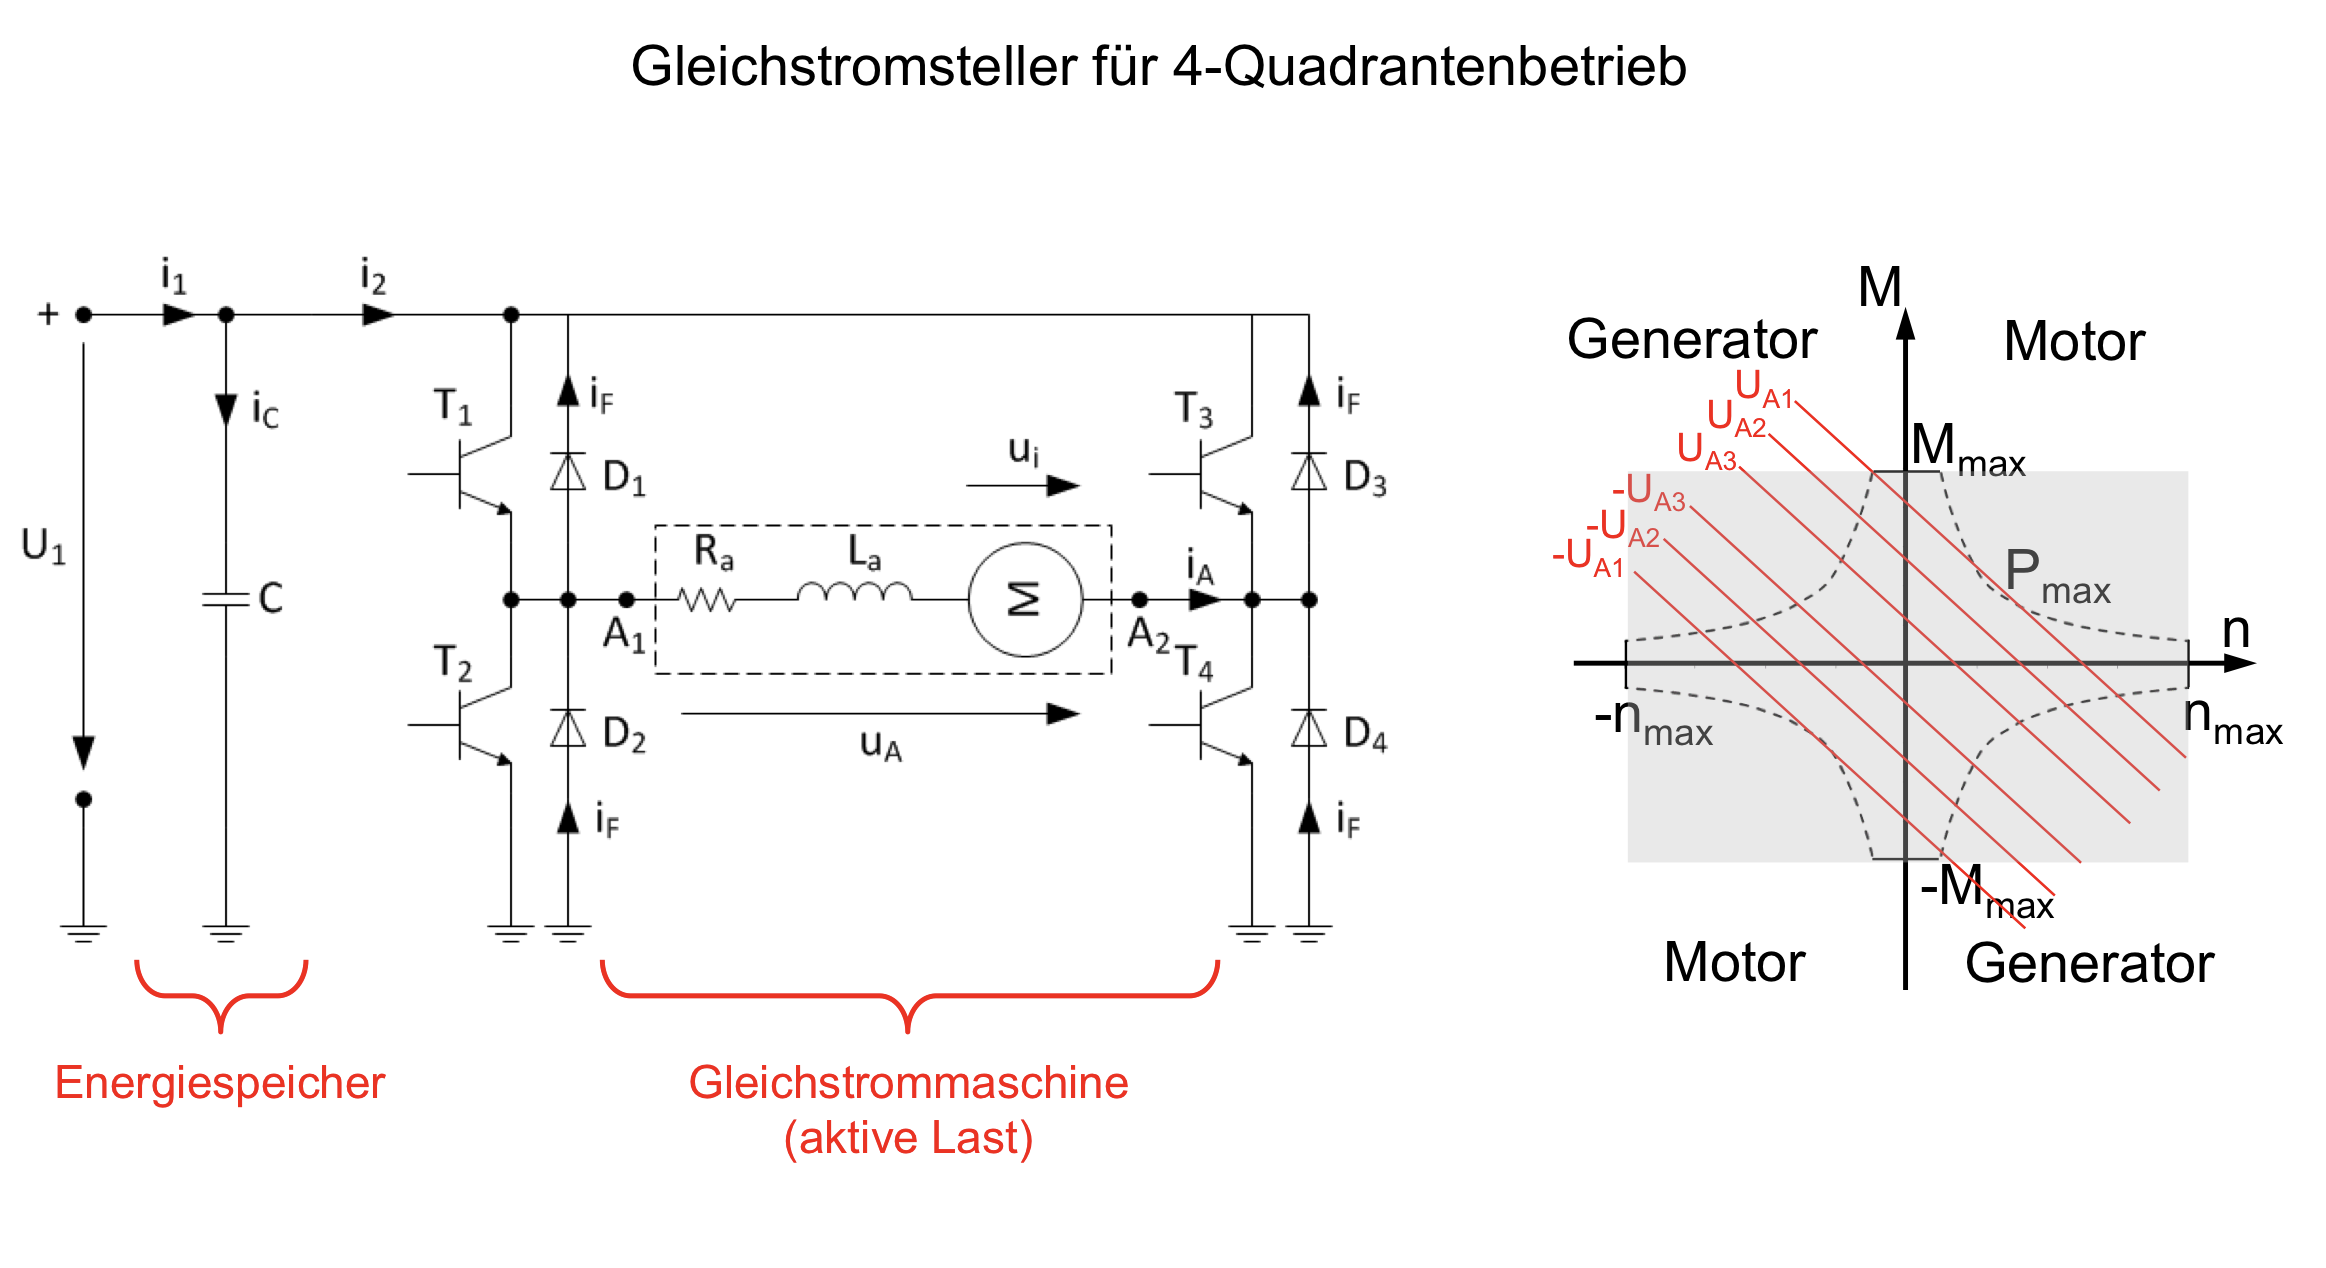
\includegraphics[width=0.85\linewidth]{images/Gleichstromsteller4Q.png}
\end{center}

Der Vierquadrantensteller erlaubt Spannungs- und Stromumkehr.
Er ermöglicht Motor- und Generatorbetrieb in beiden Drehrichtungen.
Damit sind Vorwärts- und Rückwärtslauf sowie Bremsbetrieb möglich.
Diese Topologie ist die vollständigste Form des Gleichstromstellers.
Sie wird in Reversierantrieben und Positioniersystemen eingesetzt.

Betriebsbereich:
\[
\boxed{
u_d \text{ vorzeichenwechselnd},
\qquad
i_d \text{ vorzeichenwechselnd}
}
\]

Quadranten:
\[
\begin{aligned}
\text{I:} &\; u>0,\; i>0 \quad \text{Motor vorwärts},\\
\text{II:} &\; u<0,\; i>0 \quad \text{Generator vorwärts},\\
\text{III:} &\; u<0,\; i<0 \quad \text{Motor rückwärts},\\
\text{IV:} &\; u>0,\; i<0 \quad \text{Generator rückwärts}.
\end{aligned}
\]

% -------------------------------------------------
\subsubsection{Bezug zur Gleichstrommaschine}

Ankergleichung:
\[
\boxed{u_d=R_a i_a+k\Phi\omega}
\]

Drehmoment:
\[
\boxed{M=k\Phi i_a}
\]

Drehzahl:
\[
\boxed{\omega=\frac{u_d-R_a i_a}{k\Phi}
\approx \frac{u_d}{k\Phi}}
\]

Eigenschaften:
\begin{itemize}
\item $d\uparrow \Rightarrow u_d\uparrow \Rightarrow \omega\uparrow$,
\item $d\downarrow \Rightarrow u_d\downarrow \Rightarrow \omega\downarrow$,
\item Gleichstromsteller ist das Standard-Stellglied für DC-Antriebe.
\end{itemize}


% =========================================================
\subsection{Vergleich AC-Steller -- DC-Steller}

\begin{center}
\begin{tabular}{l|c|c}
 & AC-Steller & DC-Steller \\ \hline
Spannung & Wechselspannung & Gleichspannung \\
Stellgrösse & Zündwinkel $\alpha$ & Tastgrad $d$ \\
Schaltfrequenz & Netzfrequenz & \cbl{hoch} \\
Last & R, R--L & \cbl{R--L} \\
Hauptanwendung & Heizung, Licht & \cbl{Antriebe} \\
\end{tabular}
\end{center}
